\documentclass{beamer}
\mode<presentation>
\usepackage{amsmath,amssymb,mathtools}
\usepackage{textcomp}
\usepackage{gensymb}
\usepackage{adjustbox}
\usepackage{subcaption}
\usepackage{enumitem}
\usepackage{multicol}
\usepackage{listings}
\usepackage{url}
\usepackage{graphicx} % <-- needed for images
\def\UrlBreaks{\do\/\do-}

\usetheme{Boadilla}
\usecolortheme{lily}
\setbeamertemplate{footline}{
  \leavevmode%
  \hbox{%
  \begin{beamercolorbox}[wd=\paperwidth,ht=2ex,dp=1ex,right]{author in head/foot}%
    \insertframenumber{} / \inserttotalframenumber\hspace*{2ex}
  \end{beamercolorbox}}%
  \vskip0pt%
}
\setbeamertemplate{navigation symbols}{}

\lstset{
  frame=single,
  breaklines=true,
  columns=fullflexible,
  basicstyle=\ttfamily\tiny   % tiny font so code fits
}

\numberwithin{equation}{section}

% ---- your macros ----
\providecommand{\nCr}[2]{\,^{#1}C_{#2}}
\providecommand{\nPr}[2]{\,^{#1}P_{#2}}
\providecommand{\mbf}{\mathbf}
\providecommand{\pr}[1]{\ensuremath{\Pr\left(#1\right)}}
\providecommand{\qfunc}[1]{\ensuremath{Q\left(#1\right)}}
\providecommand{\sbrak}[1]{\ensuremath{{}\left[#1\right]}}
\providecommand{\lsbrak}[1]{\ensuremath{{}\left[#1\right.}}
\providecommand{\rsbrak}[1]{\ensuremath{\left.#1\right]}}
\providecommand{\brak}[1]{\ensuremath{\left(#1\right)}}
\providecommand{\lbrak}[1]{\ensuremath{\left(#1\right.}}
\providecommand{\rbrak}[1]{\ensuremath{\left.#1\right)}}
\providecommand{\cbrak}[1]{\ensuremath{\left\{#1\right\}}}
\providecommand{\lcbrak}[1]{\ensuremath{\left\{#1\right.}}
\providecommand{\rcbrak}[1]{\ensuremath{\left.#1\right\}}}
\theoremstyle{remark}
\newtheorem{rem}{Remark}
\newcommand{\sgn}{\mathop{\mathrm{sgn}}}
\providecommand{\abs}[1]{\left\vert#1\right\vert}
\providecommand{\res}[1]{\Res\displaylimits_{#1}}
\providecommand{\norm}[1]{\lVert#1\rVert}
\providecommand{\mtx}[1]{\mathbf{#1}}
\providecommand{\mean}[1]{E\left[ #1 \right]}
\providecommand{\fourier}{\overset{\mathcal{F}}{ \rightleftharpoons}}
\providecommand{\system}{\overset{\mathcal{H}}{ \longleftrightarrow}}
\providecommand{\dec}[2]{\ensuremath{\overset{#1}{\underset{#2}{\gtrless}}}}
\newcommand{\myvec}[1]{\ensuremath{\begin{pmatrix}#1\end{pmatrix}}}
\let\vec\mathbf

\title{Matgeo Presentation - Problem 3.2.4}
\author{ee25btech11063 - Vejith}

\begin{document}


\frame{\titlepage}
\begin{frame}{Question}
Construct the triangle BD$^{\prime}$C$^{\prime}$ similar to $\triangle$BDC with scale factor $\frac{4}{3}$.Draw the line segment D$^{\prime}$A$^{\prime}$ parallel to DA where A$^p$rime lies on extended side BA.Is A$^{\prime}$BC$^{\prime}$D$^{\prime}$ a parallelogram?
\end{frame}

\begin{frame}{Description}
\textbf{Solution: }\\
\begin{table}[h!]    
  \centering
  \begin{tabular}[12pt]{ |c| c|}
    \hline
      \textbf{Vector} & \textbf{Name}\\ 
      \hline
      \myvec{0\\0} & Vector $\Vec{A}$\\
      \hline
      \myvec{4\\0} & Vector $\Vec{B}$\\
      \hline
      \myvec{4\\3} & Vector $\Vec{C}$\\
      \hline
      \myvec{0\\3} &  Vector $\Vec{D}$\\
      \hline
      \end{tabular}
  \caption{Variables Used}
  \label{}
\end{table}
\end{frame}

\begin{frame}{Solution}
consider $\triangle$BDC.constructs a $\triangle$BD$^{\prime}C^{\prime}$
 with scale factor $\frac{4}{3}$.\\
This means 
\begin{align}
  \triangle BD^{\prime}C^{\prime} \sim \triangle BDC.\\
\frac{\norm{\vec{D^{\prime}}-\vec{B}}}{\norm{\vec{D}-\vec{B}}} \;=\; \frac{\norm{\vec{C^{\prime}}-\vec{B}}}{\norm{\vec{C}-\vec{B}}} \;=\; \frac{\norm{\vec{C^{\prime}}-\vec{D^{\prime}}}}{\norm{\vec{C}-\vec{D}}} \;=\; \frac{4}{3}.\\
\Vec{D^{\prime}}=\Vec{B}+\frac{4}{3}(\Vec{D}-\Vec{B})\\
\Vec{D^{\prime}}=\myvec{-4/3\\4}\\
\Vec{C^{\prime}}=\Vec{B}+\frac{4}{3}(\Vec{C}-\Vec{B})\\
\Vec{C^{\prime}}=\myvec{4\\4}
\end{align}

\textbf{Construct A$^{\prime}$}\\
Mark $\vec{D^{\prime}}$ and $\vec{A^{\prime}}$ parallel to $\vec{D}-\vec{A}$ with $\vec{A^{\prime}}$ along the direction of  $\vec{B}-\vec{A}$.\\
\end{frame}

\begin{frame}{Solution}
\begin{align}
\vec{A^{\prime}-D^{\prime}}=\lambda(\vec{A}-\vec{D})\\
\vec{A^{\prime}}=\myvec{-4/3\\4}+\lambda(\myvec{0\\-3})\\
\implies \vec{A^{\prime}}=\myvec{-4/3\\4-3\lambda}
\end{align}
 $\vec{A^{\prime}}$ lies on line through $\vec{B}-\vec{A}$ so,
 \begin{align}
 \vec{A^{\prime}}=\vec{B}+\mu(\vec{A}-\vec{B})\\
 \implies \vec{A^{\prime}}=\myvec{-4\mu\\0}\\
 \end{align}
 From equation (0.9) and (0.11)
 \begin{align}
 \lambda=4/3 \text{and} \mu=1/3
 \end{align}
    \end{frame}
    \begin{frame}{Solution}
\begin{align}
 \implies \vec{A^{\prime}}=\myvec{-4/3\\0}\\
    \Vec{B}-\Vec{A}=\myvec{4\\0}-\myvec{0\\0}=\myvec{4\\0}\\
    \Vec{C}-\Vec{D}=\myvec{4\\3}-\myvec{0\\3}=\myvec{4\\0}\\
\implies \Vec{B}-\Vec{A}=\Vec{C}-\Vec{D}
\end{align}
    \end{frame}
    
\begin{frame}{Solution}
\textbf{Check the parallelogram property of A$^{\prime}$BC$^{\prime}$D$^{\prime}$ }\\
\begin{align}
    \vec{B}-\vec{A^{\prime}}=-t(\vec{A}-\vec{B})\\
    \vec{D^{\prime}}-\vec{C^{\prime}}=k(\vec{C}-\vec{D})\\
    \text{From 0.17 }\Vec{B}-\Vec{A}=\Vec{C}-\Vec{D}\\
\implies \vec{B}-\vec{A^{\prime}}=-t(\vec{A}-\vec{B})=t(\vec{C}-\vec{D})=\frac{t}{k}\vec{D^{\prime}}-\vec{C^{\prime}}\\
\implies \vec{B}-\vec{A^{\prime}} \parallel \vec{D^{\prime}}-\vec{C^{\prime}}
\end{align}
\text{By construction of A$^{\prime}$} 
    \begin{align}
    \vec{D^{\prime}}-\vec{A^{\prime}} \parallel \vec{D}-\vec{A}\\
    \vec{D}-\vec{A} \parallel \Vec{C}-\vec{B}\\
     \Vec{C}-\vec{B} \parallel \Vec{C^{\prime}}-\Vec{B}\\
\implies \vec{D^{\prime}}-\vec{A^{\prime}} \parallel \Vec{C^{\prime}}-\Vec{B}
\end{align}
\end{frame}

\begin{frame}{Conclusion and plot}
$\implies$A$^{\prime}$BC$^{\prime}$D$^{\prime}$ a parallelogram
\begin{figure}[H]
    \centering
    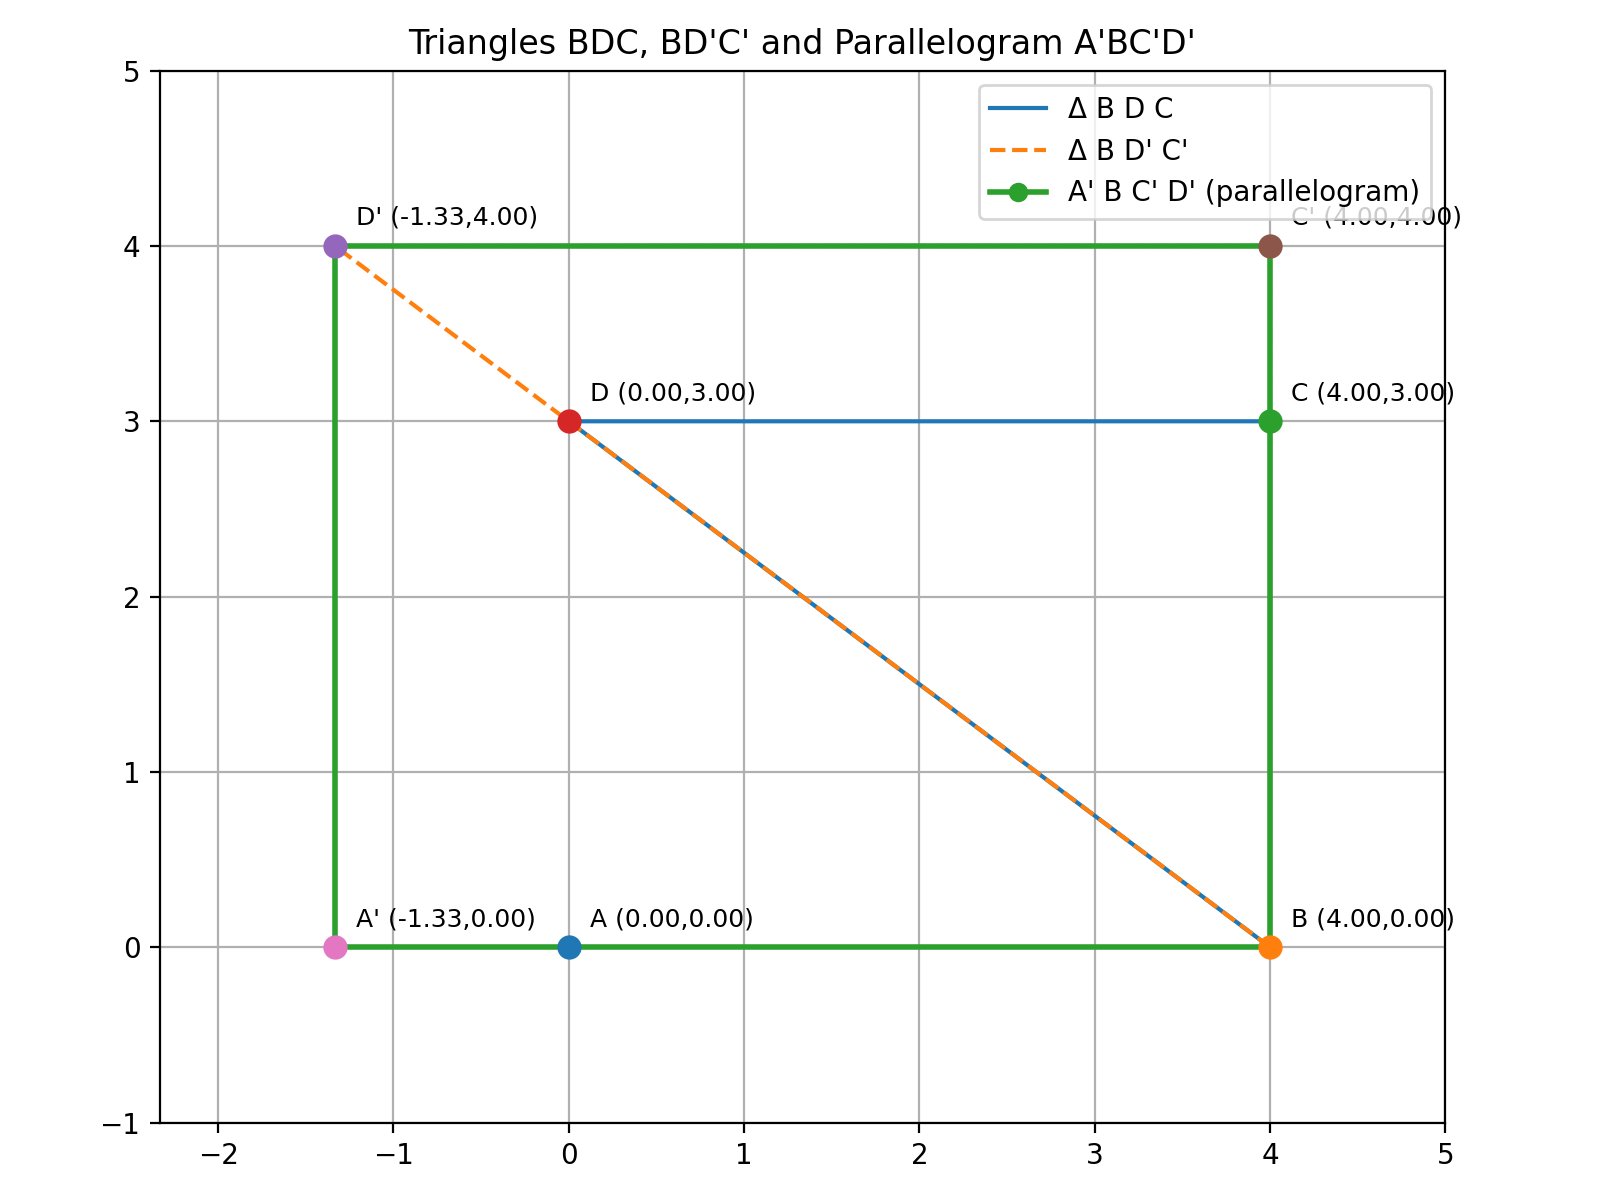
\includegraphics[width=1.0\columnwidth]{figs/01.png}
    \label{fig-1}
\end{figure}
\end{frame}


% --------- CODE APPENDIX ---------
\section*{Appendix: Code}

% C program
\begin{frame}[fragile]{C Code: triangle.c}
\begin{lstlisting}[language=C]
/* triangle.c
   - writes points to "triangle.dat"
   - computes A' so that D'A' || DA and A' lies on extended BA
   - checks whether A' B C' D' is a parallelogram
*/
#include <stdio.h>
#include <math.h>

typedef struct { double x, y; } Point;

int areParallel(Point p1, Point p2, Point q1, Point q2) {
    double dx1 = p2.x - p1.x, dy1 = p2.y - p1.y;
    double dx2 = q2.x - q1.x, dy2 = q2.y - q1.y;
    return fabs(dy1 * dx2 - dy2 * dx1) < 1e-8;
}

int main(void) {
    FILE *fp = fopen("triangle.dat", "w");
    if (!fp) {
        perror("fopen");
        return 1;
    }

    /* Choose ABCD to be a parallelogram (so final shape will be a parallelogram).
       Example: rectangle/parallelogram with A=(0,0), B=(4,0), D=(0,3).
       Then C = B + D - A = (4,3).
    */
    Point A = {0.0, 0.0};
    Point B = {4.0, 0.0};
    Point D = {0.0, 3.0};
    Point C = { B.x + D.x - A.x, B.y + D.y - A.y }; /* ensures ABCD is parallelogram */

    double k = 4.0 / 3.0;
\end{lstlisting}
\end{frame}

\begin{frame}[fragile]{C Code: triangle.c}
\begin{lstlisting}[language=C]
    /* BD'C' similar to BDC with scale factor k: D' = B + k*(D - B), C' = B + k*(C - B) */
    Point Dp = { B.x + k * (D.x - B.x), B.y + k * (D.y - B.y) };
    Point Cp = { B.x + k * (C.x - B.x), B.y + k * (C.y - B.y) };

    /* Solve for t where A' = B + t*(A - B) and D'A' || DA.
       Derivation:
         Let v = A - D.
         Let u(t) = (B - D') + t*(A - B).  (u = A' - D')
         Parallel condition: u.x * v.y - u.y * v.x = 0
       => t = [ (B.y - D'.y)*v.x - (B.x - D'.x)*v.y ]
              / [ (A.x - B.x)*v.y - (A.y - B.y)*v.x ]
    */
    double vx = A.x - D.x;
    double vy = A.y - D.y;
    double numerator  = (B.y - Dp.y) * vx - (B.x - Dp.x) * vy;
    double denominator = (A.x - B.x) * vy - (A.y - B.y) * vx;

    if (fabs(denominator) < 1e-12) {
        fprintf(stderr, "Denominator ~ 0: can't find unique A' (degenerate configuration)\n");
        fclose(fp);
        return 1;
    }

    double t = numerator / denominator;
    Point Ap = { B.x + t * (A.x - B.x), B.y + t * (A.y - B.y) };

    /* Write coordinates */
    fprintf(fp, "A  = (%.6f, %.6f)\n", A.x, A.y);
    fprintf(fp, "B  = (%.6f, %.6f)\n", B.x, B.y);
    fprintf(fp, "C  = (%.6f, %.6f)\n", C.x, C.y);
    fprintf(fp, "D  = (%.6f, %.6f)\n", D.x, D.y);
    fprintf(fp, "D' = (%.6f, %.6f)\n", Dp.x, Dp.y);
    fprintf(fp, "C' = (%.6f, %.6f)\n", Cp.x, Cp.y);
    \end{lstlisting}
\end{frame}

\begin{frame}[fragile]{C Code: triangle.c}
\begin{lstlisting}[language=C]
    fprintf(fp, "A' = (%.6f, %.6f)\n", Ap.x, Ap.y);

    /* Check parallelogram: opposite sides parallel */
    int cond1 = areParallel(Ap, B, Dp, Cp); /* A'B || D'C' */
    int cond2 = areParallel(Ap, Dp, B, Cp); /* A'D' || B C' */

    if (cond1 && cond2) {
        fprintf(fp, "\nA'BC'D' is a parallelogram.\n");
        printf("A'BC'D' is a parallelogram.\n");
    } else {
        fprintf(fp, "\nA'BC'D' is NOT a parallelogram.\n");
        printf("A'BC'D' is NOT a parallelogram.\n");
    }

    fclose(fp);
    return 0;
}
 \end{lstlisting}
\end{frame}

\begin{frame}[fragile]{Python: plot.py}
\begin{lstlisting}[language=Python]
  import numpy as np
import matplotlib.pyplot as plt

# --- Given vertices
A = np.array([0.0, 0.0])
B = np.array([4.0, 0.0])
C = np.array([4.0, 3.0])
D = np.array([0.0, 3.0])

k = 4.0 / 3.0  # scale factor

# --- Compute C' and D' (scaled triangle BDC)
Dp = B + k * (D - B)   # D'
Cp = B + k * (C - B)   # C'

# --- A' must be such that A'BC'D' is a parallelogram
# In a parallelogram: A' = B + D' - C'
Ap = B + Dp - Cp

# --- Collect points
points = {"A":A, "B":B, "C":C, "D":D, "D'":Dp, "C'":Cp, "A'":Ap}

# --- Print coordinates
print("Corrected coordinates:")
for name, p in points.items():
    print(f"{name:3} = ({p[0]:.6f}, {p[1]:.6f})")

# --- Plotting
plt.figure(figsize=(8,6))

# Original quadrilateral ABCD
plt.plot([A[0],B[0],C[0],D[0],A[0]], [A[1],B[1],C[1],D[1],A[1]], 
         'b-', linewidth=1.5, label="ABCD")
\end{lstlisting}
\end{frame} 

\begin{frame}[fragile]{Python: plot.py}
\begin{lstlisting}[language=Python]
# Triangle B-D'-C'
plt.plot([B[0],Dp[0],Cp[0],B[0]], [B[1],Dp[1],Cp[1],B[1]], 
         'r--', linewidth=1.5, label="Δ B D' C'")

# Parallelogram A'-B-C'-D'
plt.plot([Ap[0],B[0],Cp[0],Dp[0],Ap[0]], [Ap[1],B[1],Cp[1],Dp[1],Ap[1]], 
         'g-o', linewidth=2, label="Parallelogram A' B C' D'")

# Labels
for name, p in points.items():
    plt.scatter(p[0], p[1], s=60, zorder=5)
    plt.text(p[0]+0.1, p[1]+0.1, f"{name} ({p[0]:.2f},{p[1]:.2f})", fontsize=9)

plt.gca().set_aspect('equal', adjustable='box')
plt.grid(True)
plt.legend()
plt.title("Parallelogram A' B C' D' with scaled triangle BD'C'")
plt.show()
\end{lstlisting}
\end{frame}
 \end{document}
 
